\chapter{Experimental evaluation}

TODO: Chapter description with our data repository link\footnote{\url{https://github.com/dataspecer/domain-modeling-benchmark}}


\section{Evaluation domains}

To assess the quality of the generators, we used six domains with their domain description and manually created reference domain models.
We used the reference models to evaluate the suggestions generated based on the domain descriptions.
Table \ref{tab:reference-model-size} summarizes the size of these reference models.

\begin{table}[!h]
    \scriptsize
    \centering
    \setlength{\tabcolsep}{0.5em}
    \begin{tabular}{lcccccc}
         & Aircrafts & Papers & Farming & Zoos & Colleges & Vehicles \\
    \toprule
    \addlinespace
         \# classes      & 8  & 7  & 14 & 14 & 63 & 66 \\
         \# attributes   & 10 & 12 & 15 & 26 & 14 & 72 \\
         \# associations & 8  & 9  & 9  & 24 & 67 & 46 \\
    \addlinespace
    \bottomrule
    \addlinespace
    \end{tabular}
    \caption{The size of the reference domain models}
    \label{tab:reference-model-size}
\end{table}


We categorize the domains into two groups.
The first group contains three domains: \emph{aircraft manufacturing}, \emph{conference papers}, and \emph{farming}.
They are characterized by simpler descriptions with a limited scope of concepts.
For each domain, we manually created three semantically equivalent domain descriptions in three different styles.
\emph{Analytical} descriptions are written with analytical precision, describing each concept rigorously, unambiguously, and preferably with a consistent sequence of sentences.
\emph{Eclectic} are written as a collection of less structured knowledge from different stakeholders, each describing the domain from a different point of view.
\emph{Educational} emphasize the most important concepts at the beginning, where only essential aspects are described, followed by adding more details about the concepts later in the description.

Additionally, to assess the quality of our domain description filtering approaches, for each domain description we also manually created corresponding annotated domain description. In each annotated domain descriptions are tags that for each domain element from corresponding reference domain model determine the text that the corresponding domain element can be inferred from. Here is an example of the original domain description and the corresponding annotated domain description from the \emph{farming} domain: \\

\noindent{}Domain description: \textit{A farmer is an individual engaged in agriculture, growing and harvesting crops, and is identified uniquely by a name that is used to refer to the farmer from various documentation, statistical reporting, etc.} \\

\noindent{}Annotated domain description: \textit{\textbf{<farmer>}A farmer is an individual engaged in agriculture, growing and harvesting crops\textbf{</farmer>}, and \textbf{<name>}is identified uniquely by a name that is used to refer to the farmer from various documentation, statistical reporting, etc.\textbf{</name>}}

The corresponding reference model contains class ``farmer'' with the attribute ``name''. The annotated text captures that the class ``farmer'' can be inferred from the text in between the opening tag ``\textbf{<farmer>}'' and the closing tag ``\textbf{</farmer>}'': ``A farmer is an individual engaged in agriculture, growing and harvesting crops''. Similarly, the attribute ``name'' can be inferred from the text in between the opening tag ``\textbf{<name>}'' and the closing tag ``\textbf{</name>}'': ``is identified uniquely by a name that is used to refer to the farmer from various documentation, statistical reporting, etc.''.

The annotated domain description can contain multiple tags with the same name. Tags with different names can cross each other but always in a way that after a opening tag follows the corresponding closing tag with the same name.


\section{Domain description filtering evaluation}

\subsection{Evaluation methodology}


\subsubsection{Recall}

For a domain element $e$ let $Y_e$ be the set of expected relevant sentences that are marked by the tag with the name equal to $name(e)$. Let $X_e \subseteq Y_e$ be the set of sentences from $Y_e$ that our RAG algorithm marked as relevant. Then the recall $R_e$ for the domain element $e$ is computed as:

\[ R_e = \dfrac{|Y_e|}{|X_e|}, \]

\noindent{}where $|Y_e|$ denotes the size of the set $Y_e$ and $|X_e|$ denotes the size of the set $X_e$.

Now when given a domain description with it's reference domain model containing set of domain elements denoted by $E$. The recall $R$ is computed as:

\[ R = \sum_{e \in E} \dfrac{|Y_e|}{|X_e|}. \]


\subsubsection{Precision}

For a class $c$ and domain description $T$ let $Y_c$ be the set of expected relevant sentences for the class $c$, for all it's attributes and for all it's associations. Now let $Z_c$ be the set of remaining sentences from the given domain description after the filtering based on the class $c$. Then the precision $P_c$ is for the class $c$ and the domain description $T$ is computed as:

\[ P_c = \dfrac{|Y_c|}{|Z_c|}. \]

Now when given a domain description $T$ with it's reference domain model containing set of classes denoted by $C$. The precision $P$ is computed as:

\[ P = \sum_{c \in C}\dfrac{|Y_c|}{|Z_c|}. \]


%\subsubsection{$F_1$ score}

%For given recall $R$ and precision $P$ we use the classic $F_1$ score definition:

%\[ F_1 = \dfrac{2 \cdot P \cdot R}{P + R}.\]


\subsection{Limitations}

There is no strict definition on what the original text should contain for a corresponding domain element and a domain description. Therefore even when the recall is not $1.00$ it does not mean that the LLM will not be able to infer the corresponding domain element. \\

TODO: Example \\


\subsection{Results}

In the section \ref{texts_comparison} we introduced the syntactic and semantic approach for domain description filtering. For comparing these approaches now we also introduce the no-filtering approach where the domain description is not filtered at all. Here are the measured results:

\begin{table}[!h]
    \scriptsize
    \centering
    \setlength{\tabcolsep}{0.5em}
    \begin{tabular}{lcccc}

    \toprule
         & Recall classes & Recall attributes & Recall associations & Precision \\
    \toprule
    
    \addlinespace
         no-filtering      & 1.00  & 1.00  & 1.00 & 0.06 \\
    	 syntactic-pronouns-ignore & 0.87 & 0.79 & 0.84 & 0.55 \\
         syntactic-pronouns-naive & 0.93  & 0.91  & 0.90 & 0.49 \\
         semantic-pronouns-ignore & 1.00 & 0.98 & 0.98 & 0.10 \\
         semantic-pronouns-naive & 0.99 & 0.96 & 0.97 & 0.10 \\
    \addlinespace
    \bottomrule
    \addlinespace
    \end{tabular}
    \caption{The size of the reference domain models}
    \label{tab:filtering-results}
\end{table}

As expected, the no-filtering approach gets the highest possible score in terms of recall however, in terms of precision it gets the lowest score from all the other approaches.

In the syntactic approach we see that naive pronouns detection improves the recall significantly but slightly decreases the precision.

The semantic approach almost matches the no-filtering in terms of recall. However, it improves the precision. (TODO: Improve wording)

Overall, when recall is important then the no-filtering approach or the semantic approach can be used. On the other hand, if we do not care about LLM not showing all possible domain elements suggestions, the syntactic approach works the best.


\section{Selected LLMs}

As running a LLM requires a lot of resources, using LLM through some API typically costs some money. To have more freedom with our experiments we run open-source LLMs locally with LLaMA.cpp server\footnote{\url{https://github.com/ggerganov/llama.cpp/blob/master/examples/server/README.md}} on a single NVIDIA A100 40GB GPU.

We decided to use a pre-trained open-source LLM because training own model requires a ton of resources and fine-tuning some existing LLM requires a lot of data.

Because of our hardware limitation we use Mixtral-8x7B\footnote{\url{https://huggingface.co/TheBloke/Mixtral-8x7B-Instruct-v0.1-GGUF/blob/main/mixtral-8x7b-instruct-v0.1.Q5_K_M.gguf}} (medium sized LLM) \cite{Jiang2024} and Llama-3-70B\footnote{\url{https://huggingface.co/bartowski/Meta-Llama-3-70B-Instruct-GGUF/blob/main/Meta-Llama-3-70B-Instruct-Q5_K_M.gguf}} (relatively large-size LLM) both in quantized variation where on average they have 5 bits per parameter.

Mixtral-8x7B has a context window size of 32k tokens and it outperforms or matches ChatGPT-3.5 across all evaluated benchmarks. This LLM has in total 47B parameters, which are distributed among 8 experts. To achieve faster output generation, for each generated token 2 of the 8 experts are selected. The selection of the experts can be different for each token \cite{Jiang2024}.

Llama-3-70B has 8k tokens context window size and is allegedly  the first open-source LLM to match the ChatGPT-4's performance. However, as of writing this thesis, Meta's research paper about Llama 3 is not released yet.

For LLM's output comparison, we also frequently used ChatGPT-3.5 through the web UI. \\

NOTE: Potom až otestujeme i ChatGPT-4o, tak sem o tom LLM něco napíšu. \\


\section{Challenges}
\begin{itemize}
\item one element can be modeled in a various ways
\item for our purposes no existing tool for automated evaluating
\end{itemize}


\section{Limitations}
\begin{itemize}
\item we used one domain modeling expert for evaluation
\item we did preliminary experiments on most of the configurations with one shorter and one longer domain description and then used more domain descriptions for the most promising configurations
\end{itemize}


\section{Generated domain elements evaluation}
(= generated classes, attributes, associations evaluation)

TODO: subsekce se všemi těmi různými pravidly, podle kterých jsme vyhodnocovali recall a precision \\


\section{Descriptions evaluation}


\section{User-based evaluation of the application}

In addition to the measurements of the performance of the genererators, we also evaluated how real domain modelers accept an automated domain modeling assistant.

We prepared two domain descriptions, a summary of the main features of the prototype, and three 2-minute video tutorials.

We instructed real users to model the two domains and then asked them to assign a number between 0 (fully disagree) and 4 (fully agree) to express their agreement with five different claims about using our prototype tool.
They also classified themselves as teachers, students, modeling experts, database experts, programmers, or managers (multiple options were allowed).
We received responses from 18 users.

Figure \ref{fig:user-based-evaluation} shows for each type of users the number of responses that picked this type and the average marks received for that type. The last line shows the average of all users.

\begin{figure}[!h]
    %\centering
    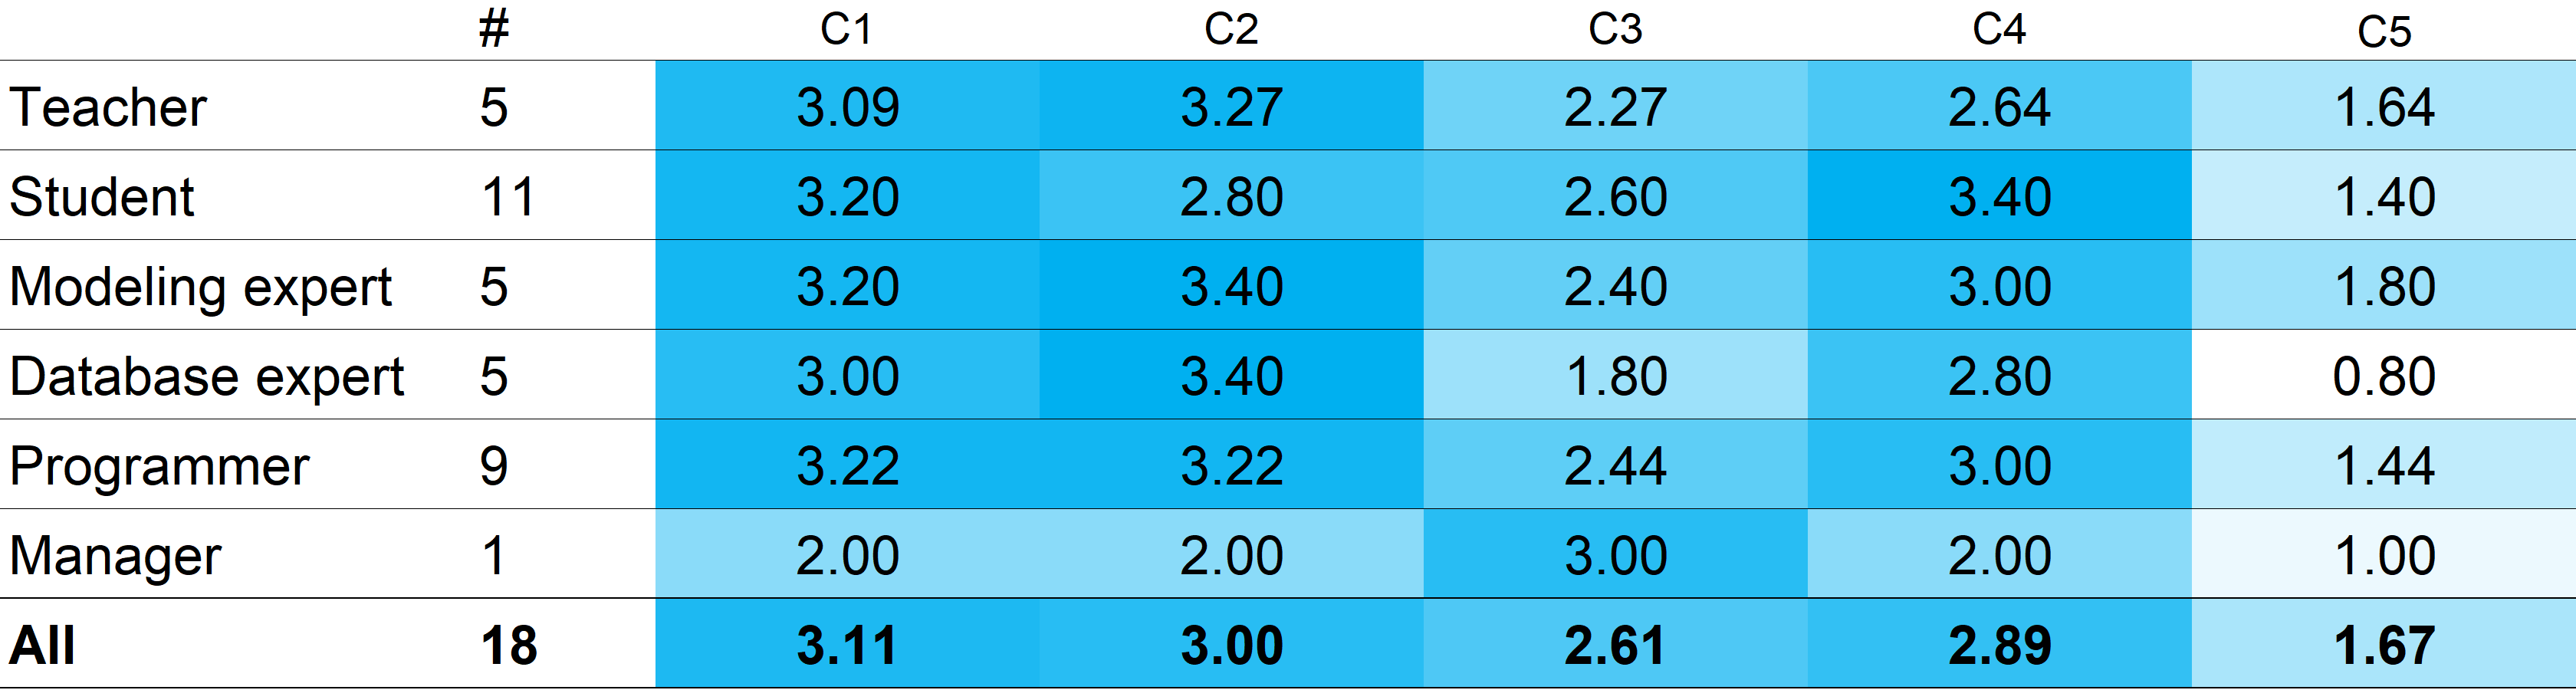
\includegraphics[width=1\linewidth]{img/user-based-evaluation.png} \\
    \scriptsize
\raggedright{C1: Modeling with the assistant is better compared to manual modeling. \\
C2: The assistant is intuitive to use.\\
C3: The assistant suggests appropriate classes, attributes, and associations.\\
C4: The assistant helped me solve the tasks faster compared to manual modeling.\\
C5: I solved all the tasks using only the assistant, and manual modeling was not needed.}
    \caption{Summary of the user-based evaluation. 0=fully disagree, 4=fully agree.}
    \label{fig:user-based-evaluation}
\end{figure}

As we can see, the users agree that using the automated assistant is better than pure manual modeling (C1) and found it intuitive (C2).
The suggestions provided by the tool are subjectively not always appropriate (Q3), which is also supported by our measurements presented in the previous part, and manual modeling is still necessary (Q5).
Despite these imperfections, users claimed that the prototype made them more productive (Q4).
We can find the weakest support in the manager category, but we were able to get only one response in this category, so a further evaluation is necessary.